\documentclass[main.tex]{subfiles}
\begin{document}
流变学(rheology)在牛津语言网站上的释义是:研究物质的变形和流动——特别是液体的非牛顿流动和固体的塑性流动——的科学(The branch of science that deals with the deformation and flow of matter, esp. the non-Newtonian flow of liquids and the plastic flow of solids)。

流变学是一门力学,属于经典力学范畴。力学包括静力学(statics)、运动学(kinematics)和动力学(dynamics)三种问题。静力学集中考虑物体处于力的平衡之下的问题。运动学定量描述物体的位置和状态随时间的变化关系。动力学研究和分析物体运动状态改变的原因。\cite[p.~1]{邓文基2009大物上}

\begin{wrapfigure}{R}{0.25\textwidth}
\centering
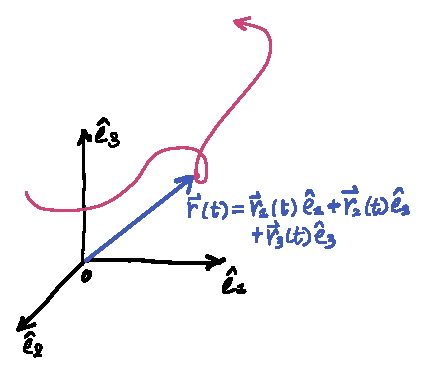
\includegraphics[width=0.25\textwidth]{images/I.1.1.eps}
\caption{质点运动学}
\label{fig:I.1.1}
\end{wrapfigure}

在经典力学的运动学中,为了描述物体的位置,我们需要先选择参考系(frame of reference),建立坐标系(coordinates),使用位置向量来表示质点的位移。我们假设时间是连续的,把质点的位移写成时间的函数,在可导的前提下,其速度和加速度分别是位移的一阶和二阶时间导数\cite[附录A,p.~422]{邓文基2009大物上}(如图\ref{fig:I.1.1}所示):
\begin{align*}
\mathbf{r}&=\mathbf{r}\left(t\right)=r_1\mathbf{\hat{e}}_1+r_2\mathbf{\hat{e}}_2+r_3\mathbf{\hat{e}}_3,\\
\mathbf{v}&=\frac{d\mathbf{r}}{dt},\mathbf{a}=\frac{d^2\mathbf{r}}{dt^2}
\end{align*}

经典力学的动力学遵循牛顿运动定律,引入了“力”的概念作为物体运动状态变化的原因(第一定律),并建立了定量关系(第二定律),以及一个守恒律(第三定律)。牛顿运动定律在且仅在惯性系下成立。作为质点的动力学,在选定惯性系下,
\[\mathbf{F}=m\frac{d\mathbf{v}}{dt}\]
其中$m$是质点的质量,是惯性(改变物定运动状态的代价)大小的量度。上式可以推广到多个质点的体系,

对于一个可以发生形变和流动的物体,上述的质点运动学和动力学在描述形变和流动问题中是不够用的。

以下是两种适用的力学:
\begin{itemize}
    \item 连续介质力学(continuum mechanics):把宏观物体视为可无限微分的连续体。从热力学基本定律和牛顿运动定律(惯性系)出发,建立物体运动与形变的本构关系。
    \item 统计力学(statistical mechanics):考虑组成物质的微观粒子的运动规律,基于统计力学的假设推出宏观物体的本构关系。高分子物理中,从链统计出发建立的粘流模型和橡胶弹性模型就是统计力学在高分子物理中的应用。
\end{itemize}

描述宏观物体形变规律的语言是连续介质力学。统计力学只是进一步给出微观原因,它关于宏观规律的预测仍旧要使用连续介质力学的语言来表述。

在连续介质力学中,一个物体的独特力学性质,是由它的本构关系/方程(constitutive relation/equation)来描述的。在一般物理学中,本构关系是指描述物质对外场激励的响应的定量关系:外场$\mathcal{S}\left(\mathbf{r},t\right)\rightarrow$材料特性函数$\mathcal{G}\left(\Delta\mathbf{x},\Delta t\right)\rightarrow$材料响应$\mathcal{R}\left(\mathbf{x},t\right)$。其中,$\mathbf{r}$是空间任一位置,$\mathbf{x}$是处于材料内部的某位置。$\mathcal{G}\left(\Delta\mathbf{x},\Delta t\right)$是材料本身的性质,称为物料函数(material function)。我们留意到,$\mathcal{S}$和$\mathcal{R}$都是场函数。物料函数是对材料观测的时间和空间间隔的函数,在数学形式上也是场函数\cite[\S~9.7,p.192]{华工高数2009下}。以下我们通过两个例题来理解本构关系的概念。这两个例题都是以前的课程中介绍过的,请注意参见例中标注的引用。

\begin{figure}[h]
\centering
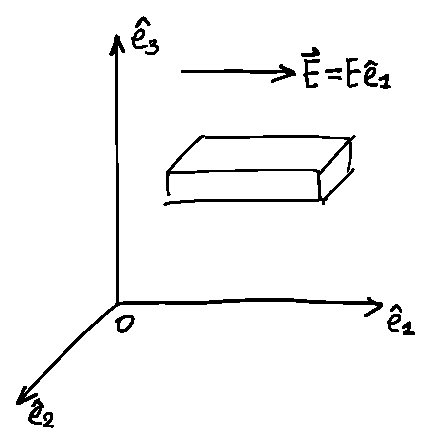
\includegraphics[width=0.25\textwidth]{images/I.1.2.eps}
\caption{例\ref{exp:I.1.1}}
\label{fig:I.1.2}
\end{figure}

\begin{example}\label{exp:I.1.1}
此例中,外场是稳恒电场$\mathbf{E}\left(\mathbf{r},t\right)=\mathbf{E}=E\mathbf{\hat{e}}_1$,材料的物性函数是电极化率$\chi\left(\Delta\mathbf{x},\Delta t\right)$(如图\ref{fig:I.1.2}所示)。对于各向同性均匀材料$\chi=\text{const}$。材料的响应是电极化强度密度$\mathbf{P}\left(\mathbf{x},t\right)$,表示材料内$\mathbf{x}$处单位体积的电极化强度,即$\mathbf{P}\left(\mathbf{x},t\right)dV$表示$\mathbf{x}$处的微体积$dV$的电极化强度。实验表明,当电场不太大时\cite[\S18.2.3,p.~57]{邓文基2009大物下},
\[
\mathbf{P}\left(\mathbf{x},t\right)=\chi\varepsilon_0\mathbf{E}\left(\mathbf{r}=\mathbf{x},t\right)
\]
其中$\varepsilon_0$是真空电容率。故本例中
\[
\mathbf{P}\left(\mathbf{x},t\right)=\chi\varepsilon_0 E\mathbf{\hat{e}}_1
\]
这是该材料的电极化本构方程。
\end{example}

\begin{example}\label{exp:I.1.2}
此例中外场是一个梯度场,例如温度场$T\left(\mathbf{r},t\right)=kr_1\mathbf{\hat{e}}_1,\nabla T\left(\mathbf{r},t\right)=k\mathbf{\hat{e}}_1$。材料的物料函数是传输物料函数,例如热导率$\kappa=\text{const}$(假设各向同性均匀材料)。材料的响应是流(flux),即单位时间经过$\mathbf{x}$处面积元$\mathbf{n}dS$的物理量。例如热流:$\mathbf{q}\left(\mathbf{x},t\right)$,$\mathbf{q}\left(\mathbf{x},t\right)\cdot\mathbf{n}dS$是单位时间通过面积元$\mathbf{n}dS$的热量。$\mathbf{q}$的方向与等温面垂直并指向温度减小的方向。实验表明,当温度梯度不太大时,热流满足傅立叶热传导定律\cite[\S1.1.3.1,p.~9]{钟理化工原理上册2008}:
\[
\mathbf{q}\left(\mathbf{x},t\right)=-\kappa\nabla T\left(\mathbf{r}=\mathbf{x},t\right)=-k\kappa\mathbf{\hat{e}}_1
\]
这是该材料的热传导本构方程。
\end{example}

流变学中的本构关系主要是应力与应变(或应变速率)的关系。

\begin{figure}[h]
\centering
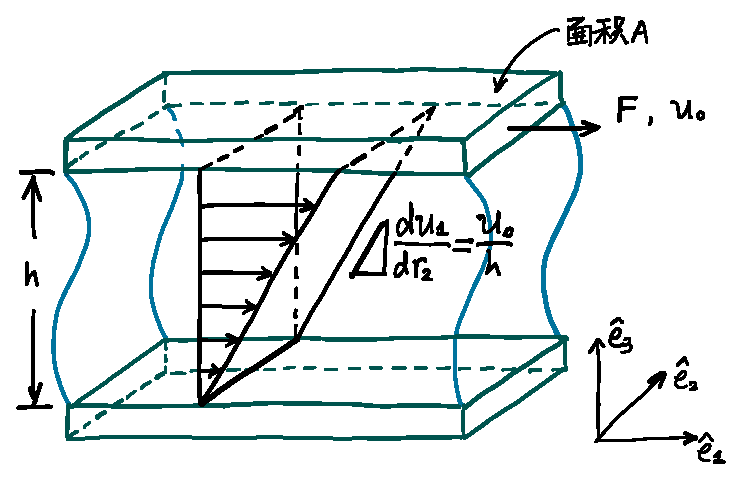
\includegraphics[width=0.5\textwidth]{images/I.1.3.eps}
\caption{例\ref{exp:I.1.3}}
\label{fig:I.1.3}
\end{figure}

\begin{example}[简单剪切下的牛顿流体本构关系]\label{exp:I.1.3}
如图\ref{fig:I.1.3}所示的间距为$h$、面积足够大的两平行板间充满粘度为$\mu$牛顿流体。按照下板固定建立参考系,建立如图所示的坐标系。上板以速率$u_0$往平行于下板的方向运动。假设流体与平板接触的界面处相对流速为零;液体的流速$\mathbf{u}\left(\mathbf{r},t\right)=u_0r_2\mathbf{\hat{e}}_1/h$。若上板面积为$A$、所受的拖曳力大小为$F$(方向与上板运动速度相同)。$F$与$u_0$的关系是
\[
\tau=\frac{F}{A}=\mu\frac{u_0}{h}
\]
这是一个本构关系:$u_0$是外场,$F$是材料响应,$\mu$是物料函数。
\end{example}

\begin{figure}[h]
\centering
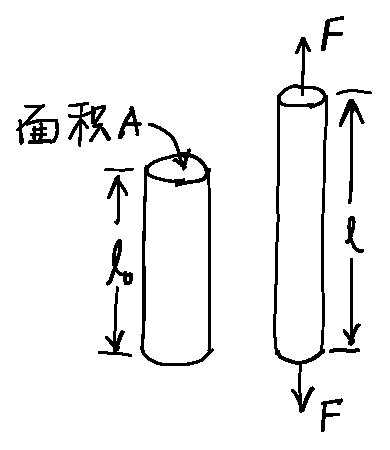
\includegraphics[width=0.25\textwidth]{images/I.1.4.eps}
\caption{例\ref{exp:I.1.4}}
\label{fig:I.1.4}
\end{figure}

\begin{example}[轴向拉伸下的虎克固体本构关系]\label{exp:I.1.4}
如图\ref{fig:I.1.4}所示的虎克固体直圆杆,弹性模量为$E$,初始截面积为$A$,初始长度为$l_0$。在杆的轴向受到大小为$F$的力时,杆的长度为$l$,则$F$与$l$的关系是
\[
\sigma=\frac{F}{A}=E\frac{l-l_0}{l_0}
\]
这是一个本构关系:$F$是外场,$l$是材料响应,$E$是物料函数。
\end{example}
上面两例中的本构方程形式只适用于特定形变方式。要完整描述一般形变过程的运动学和动力学,需要使用向量和张量以及它们的代数和微积分数学基础。

实际物体的运动和形变是在一定的初条件(initial condition)和边界条件(boundary condition)下,遵循守恒律(balance law)和本构关系的共同限定下才被具体确定的。在采用质点来简化的问题中,这些要素往往是隐含的条件。下面以一个例子说明,在解决一个具体流动问题的过程中,初条件、边界条件、守恒律和本构关系的角色。

\begin{figure}[h]
\centering
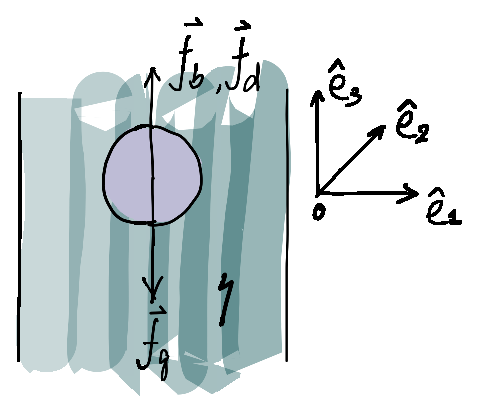
\includegraphics[width=0.25\textwidth]{images/I.1.5.eps}
\caption{落球粘度计原理图}
\label{fig:I.1.5}
\end{figure}

\begin{example}[落球粘度计]\label{exp:I.1.5}
半径为$a$的球浸没在粘度为$\eta$的牛顿流体中。以液体的容器为参考系,建立如图\ref{fig:I.1.5}所示的坐标系。球的运动满足牛顿第二定律,即:$\mathbf{F}=md\mathbf{v}/dt$(动量守恒),其中$m=\mathrm{const}$是球的质量(质量守恒)。此时,我们并不能确定球的具体运动。

设$t=0$时刻球速$\mathbf{v}=\mathbf{0}$(初条件),液体的密度为$\rho_\mathrm{w}$、球的密度为$\rho_\mathrm{s}$,则球受到的重力是$\mathbf{f}_\mathrm{g}=-4\pi\rho_\mathrm{s}ga^3\mathbf{\hat{e}}_3/3$,浮力$\mathbf{f}_\mathrm{b}=4\left(\rho_\mathrm{w}-\rho_\mathrm{s}\right)\pi ga^3\mathbf{\hat{e}}_3$,液体对球的拖曳力$\mathbf{f}_\mathrm{d}=-k\pi\eta a\mathbf{v}$(本构关系)。其中,当球面处的相对流速总为零时,$k=6$(边界条件)。由牛顿第二定律,
\[
\frac{4/3}\pi\rho_\mathrm{s}ga^3\frac{d\mathbf{v}}{dt}=\frac{4}{3}\pi ga^3\left(\rho_\mathrm{w}-\rho_\mathrm{s}\right)-6\pi\eta a\mathbf{v}
\]
解方程得:
\begin{align*}
    \mathbf{v}\left(t\right)&=v_1\left(t\right)\mathbf{\hat{e}}_1+v_2\left(t\right)\mathbf{\hat{e}}_2+v_3\left(t\right)\mathbf{\hat{e}}_3\\
    v_1\left(t\right)&=v_2\left(t\right)\equiv0\\
    v_3\left(t\right)&=\frac{2\left(\rho_\mathrm{w}-\rho_\mathrm{s}\right)ga^3}{9\eta}\left(1-e^{\frac{-9\eta t}{2\rho_\mathrm{s}a^2g}}\right)
\end{align*}
当$t\rightarrow\infty$时,
\begin{align*}
v_3\left(t\right)&\equiv v_\infty= \frac{2\left(\rho_\mathrm{w}-\rho_\mathrm{s}\right)ga^2}{9\eta}\\
\eta&=\frac{2\left(\rho_\mathrm{w}-\rho_\mathrm{s}\right)ga^2}{9v_\infty}
\end{align*}
\end{example}

上例中的考察对象(球)是刚体,在运动过程中形状不变。在流变学中,我们要描述物体在形变过程中如何保持质量、动量和能量守恒,这需要借助场函数的一系列积分定理,相关的知识将会在数学准备部分介绍。
\end{document} 
